% 
\documentclass[a4paper,10pt]{report}
\usepackage[utf8x]{inputenc}
\usepackage[OT1]{fontenc}
\usepackage{hyperref}
\usepackage{Sweave}
\usepackage{graphicx}
\usepackage{color}
\graphicspath{{figures/}}
%\usepackage{float}
\usepackage{wrapfig}
%\usepackage{subfigure}
%% Package to linebreak URLs in a sane manner.
\usepackage{url}
%% Define a new 'smallurl' style for the package that will use a smaller font.
\makeatletter
\def\url@smallurlstyle{%
  \@ifundefined{selectfont}{\def\UrlFont{\sf}}{\def\UrlFont{\small\ttfamily}}}
\makeatother
%% Now actually use the newly defined style.
\urlstyle{smallurl}
%% Define 'tinyurl' style for even smaller URLs (such as in tables)
\makeatletter
\def\url@tinyurlstyle{%
  \@ifundefined{selectfont}{\def\UrlFont{\sf}}{\def\UrlFont{\scriptsize\ttfamily}}}
\makeatother
%% Make margins less ridiculous
\usepackage{fullpage}
%% Make URLs clickable
%\usepackage[colorlinks, bookmarks=false]{hyperref}
%\usepackage[colorlinks, bookmarks=true]{hyperref}
%% Since I'm using the LaTeX Makefile that uses dvips, I need this
%% package to make URLs break nicely
\usepackage{breakurl}
\usepackage{todonotes}
\usepackage{amsmath,amsfonts}
\numberwithin{equation}{subsection}
%%\usepackage{nonfloat}
\usepackage{bbm}
\usepackage{setspace}
\onehalfspacing
\usepackage{tabularx}

%
%
%
\usepackage{listings}
\usepackage{courier}
\lstset{
         basicstyle=\footnotesize\ttfamily, % Standardschrift
         %numbers=left,               % Ort der Zeilennummern
         numberstyle=\tiny,          % Stil der Zeilennummern
         stepnumber=2,               % Abstand zwischen den Zeilennummern
         numbersep=5pt,              % Abstand der Nummern zum Text
         tabsize=2,                  % Groesse von Tabs
         extendedchars=true,         %
         breaklines=true,            % Zeilen werden Umgebrochen
         keywordstyle=\color{red},
    		frame=b,         
 %        keywordstyle=[1]\textbf,    % Stil der Keywords
 %        keywordstyle=[2]\textbf,    %
 %        keywordstyle=[3]\textbf,    %
 %        keywordstyle=[4]\textbf,   \sqrt{\sqrt{}} %
         stringstyle=\color{white}\ttfamily, % Farbe der String
         showspaces=false,           % Leerzeichen anzeigen ?
         showtabs=false,             % Tabs anzeigen ?
         xleftmargin=17pt,
         framexleftmargin=18pt,
         framexrightmargin=6pt,
         framexbottommargin=4pt,
         %backgroundcolor=\color{lightgray},
         showstringspaces=false      % Leerzeichen in Strings anzeigen ?        
 }
 \lstloadlanguages{% Check Dokumentation for further languages ...
         %[Visual]Basic
         %Pascal
         %C
         %C++
         %XML
         %HTML
         Java
 }
%\DeclareCaptionFont{blue}{\color{blue}} 
%\captionsetup[lstlisting]{singlelinecheck=false, labelfont={blue}, textfont={blue}}
\usepackage{caption}
\DeclareCaptionFont{white}{\color{white}}
\DeclareCaptionFormat{listing}{\colorbox[cmyk]{0.43, 0.35, 0.35,0.01}{\parbox{\textwidth}{\hspace{15pt}#1#2#3}}}
\captionsetup[lstlisting]{format=listing,labelfont=white,textfont=white, singlelinecheck=false, margin=0pt, font={bf,footnotesize}}
%
%

\begin{document}

\title{Mining of Android SCM}
\author{Pavel Senin}

\maketitle

\begin{abstract}
Both, software product improvement and software process improvement, require in-depth understanding 
of current project state. Here I present an approach for exploration of a software repository by 
using Software Trajectory code. I will explore Android SCM system\ldots
\end{abstract}

\section{Introduction}
According to the Android home website, \url{http://source.android.com/}: ``Android is an 
open-source software stack for mobile phones and other devices''.

Initial developer of the software, Android Inc. - a small startup company - was purchased by Google 
in in 2005. In November 2007 the Open Handset Alliance, a consortium of 84 companies, announced 
availability of the Android Software Development Kit (SDK). The open Open Handset Alliance was formed 
of hardware, software, and telecommunication companies (including Intel, HTC, ARM, Samsung and Motorola)
and devoted to advancing of open standards for mobile devices. 

\begin{wrapfigure}{l}{0.5\textwidth}
   \begin{center}
   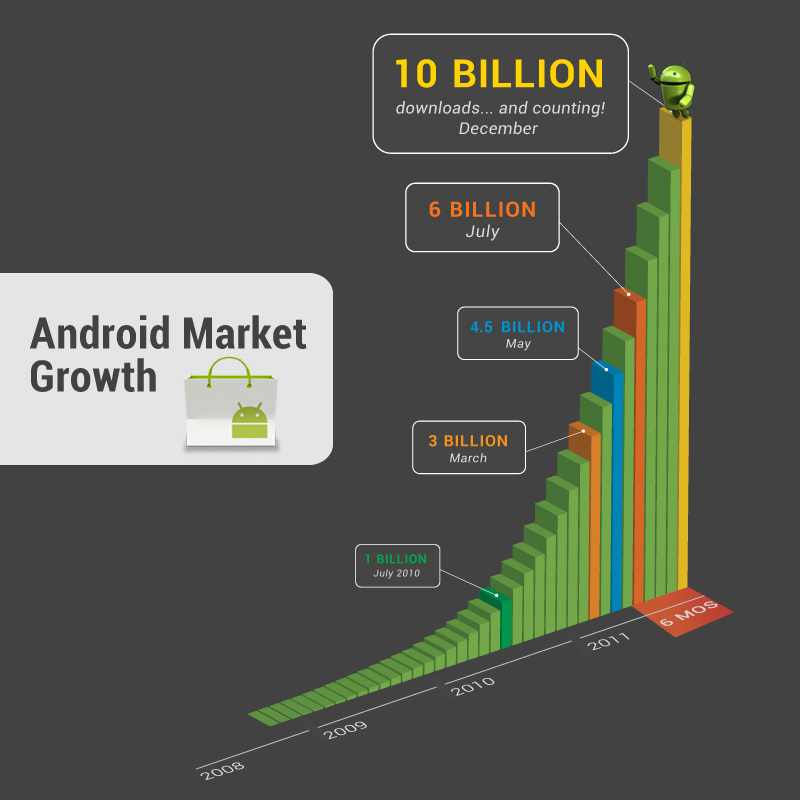
\includegraphics[scale=0.3,width=0.48\textwidth]{graph_only_3}
   \end{center}
   \caption{The Android store downloads timeline.}
   \label{fig:android_downloads}
\end{wrapfigure}

The Android code is open-source and released under the Apache License; it is a complete 
mobile platform built on the monolithic Linux 2.6 kernel. The Android platform provides 
developers with an SDK which consits of a set of development tools, debugger and a true emulator. 
There are an Eclipse plugin, a set of libraries a multimedia user interface, and a core set of 
phone applications. The Android application model alleviates the cost of software development by 
allowing extending, replacing, and reusing of existing software components. The Dalvik virtual 
machine, which is the part of Android distribution, provides a way to maximize application portability, 
performance and security. Android OS allows true application multitasking, provides rich user 
notifications and customizable home screens with resizable widgets. Latest, 4.0 version of
Android System provides streaming voice recognition.

Currently, the Android Open Source Project (AOSP) is led by Google and includes not only the 
original members of OHA but many other companies. The role of AOSP is to maintain and develop 
Android.

Including Beta, there were 10 major releases of Android as well as a number of intermediate 
releases. All releases prior to 2.0 were for mobile phones exclusively. Since 2.0 release 
Android OS is a tablet-oriented operating system. Most of the mobile devices at market use 
2.x version of Android. The 3.0 release, Honeycomb, does not officially run on phones; 
the latest 4.0 release, Ice Cream Sandwich, runs on all mobile devices.

In Q3, 2011 (November 15, 2011) Android officially become the most popular OS for newly sold mobile 
devices. In December 2011 there were registered 10 billions of downloads from Android store called
Android Marketplace. 

\section{MSR-2012}
The research field of Mining Software Repositories (MSR) is focused on analyzes of the rich 
data available in software repositories. The immediate goal of such research is to infer interesting 
and actionable information about software systems and projects. While there are multiple scientific 
events where researchers working in the field meet, the Mining Software Repositories 
conference considered to be the major meeting event. The 2012 MSR conference is a 9th such event
and is collocated with ICSE -the International Conference on Software Engineering.
Along with the research track since 2006 the MSR conference includes the Mining Challenge where 
researchers demonstrate application of their tools to the selected repository mining problem. This
year Android platform was selected for the challenge. Two XML files containing change and bug report 
data were offered to participants to uncover interesting facts related to the Android platform.

\section{Data provided, auxiliary information collection and assimilation.}
The two files offered for the research track of MSR conference contained most of the information
obtainable from Google-hosted source code repository as well as Google-hosted bug and issue
tracking system. The full XSD for both XML files can be found in the Appendix section of this report.
While the issues and comments trail \ref{bugsXSD} was provided nearly complete,
the change trail \ref{changeXSD} provided for a challenge contained only the high-level information as 
shown at \ref{changeXSDFragment}. (i need to mention the specificity of what Trajectory is capable of
to show the limitation imposed by incomplete data)
By using this data it is possible to infer the temporal activity of every repository contributor along with some quantitative data concerning the total number of changed 
targets. However the amount of information provided provided change it offers some projection 
\lstset{label=changeXSDFragment,caption=List of metadata provided by change trail XML (fragment) }
\begin{lstlisting}
 <xs:element name="change">
    <xs:complexType>
      <xs:sequence>
        <xs:element ref="project"/>
        <xs:element ref="commit_hash"/>
        <xs:element ref="tree_hash"/>
        <xs:element ref="parent_hashes"/>
        <xs:element ref="author_name"/>
        <xs:element ref="author_e-mail"/>
        <xs:element ref="author_date"/>
        <xs:element ref="commiter_name"/>
        <xs:element ref="commiter_email"/>
        <xs:element ref="committer_date"/>
        <xs:element ref="subject"/>
        <xs:element ref="message"/>
        <xs:element ref="target"/>
      </xs:sequence>
    </xs:complexType>
  </xs:element>
\end{lstlisting}



There are 1771667 changes 

registered in the repository. First change commit to Android repository dates back 
to Monday January 12th 1970, 14:46:40 and belongs to Upstream, while the last change
within the analyzed data set belongs to to Guy Zadickario and dated 
Tuesday June 21st 2011, 12:41:41.


\section{Source code}
As per January, 1, 2012 Android repository contains a total of 26851267 lines of source code in 
152225 files. 

\begin{table}
  \caption{Android repository snapshot source code metrics.}
  \begin{tabularx}{\textwidth}{ | X | r | r | r | r | r |}
  \hline                       
  Nb. files & Language & Total lines & Source & Blanks & Comments \\
  \hline 
  Assembly &3391 & 565314 & 426104 & 60673 & 98215 \\
  IDL & 78 & 7926 & 7174 & 752 & 640 \\
 Perl & 348 & 105024 & 75877 & 13999 & 18975 \\    
  CSS & 224 & 38417 & 30687 & 5899 & 2033 \\
  XML & 10090 & 5963665 & 5762297 & 59093 & 143243 \\   
  Matlab & 889 & 62911 & 51323 & 10715 & 3911 \\
  Text & 7563 & 1669710 & 0 & 93271 & 1576439 \\
  FlashParameter & 3 & 364 & 265 & 40 & 59 \\
  C & 42151 & 9979284 & 6676807 & 1278259 & 2363003 \\   
  shell & 3930 & 2476537 & 1986936 & 207861 & 288125 \\  
  JavaScript & 5347 & 866236 & 511330 & 131581 & 225745 \\   
  Java & 251129 & 5265723 & 3152054 & 639535 & 1509917 \\
  HTML & 6209 & 1208415 & 1062506 & 100306 & 61760 \\
  make & 3506 & 512065 & 377850 & 62696 & 71518 \\
  Awk & 21 & 2762 & 1778 & 226 & 871 \\
  SQL & 3 & 454 & 454 & 0 & 0 \\
  Pascal & 160 & 15681 & 2555 & 372 & 13334 \\      
  Python & 912 & 190278 & 132202 & 30889 & 27888 \\ 
  PHP & 180 & 50137 & 39060 & 2268 & 9218 \\
  C++ & 31390 & 9228878 & 6262708 & 1318921 & 1835150 \\   
  Jess & 2 & 246 & 192 & 54 & 0 \\
  CSharp & 66 & 6513 & 5282 & 643 & 596 \\      
  Lisp & 10633 & 493777 & 285826 & 86471 & 176378 \\
  \hline     
  TOTAL & 152225 & 38710317 & 4104524 & 8427018 & 26851267 \\    
  \hline  
  \end{tabularx}
\end{table}

\section{MSR 2012 Challenge}

\clearpage
\lstinputlisting[label=bugsXSD,caption=Bugs XML file schema]{bugs.xsd}

\clearpage
\lstinputlisting[label=changeXSD,caption=Change XML file schema]{git.xsd}
\end{document}
